25. $\cfrac{(2x^2+x+1)(6x-x^2-9)}{x^2+8x+15}\geqslant0\Leftrightarrow \cfrac{-\left(\left(x+\cfrac{1}{2}\right)+x^2+\cfrac{3}{4}\right)(x-3)^2}{(x+3)(x+5)}\geqslant0.$ Применив метод интервалов, найдём ответ: $x\in
(-5;-3)\cup\{3\}.$
\begin{figure}[ht!]
\center{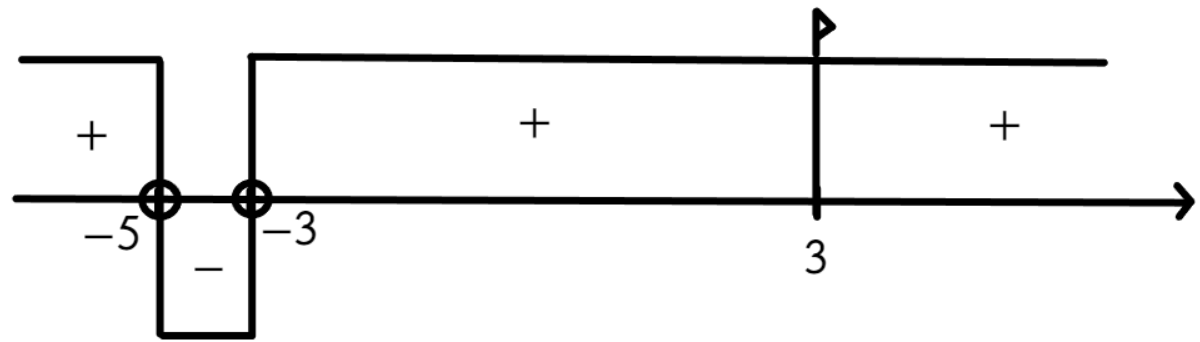
\includegraphics[scale=0.35]{ner9-25.png}}
\end{figure}\\
